\documentclass[12pt,a4paper]{report}

% ============ PACKAGES ============
\usepackage[utf8]{inputenc}
\usepackage[T1]{fontenc}
\usepackage{lmodern}
\usepackage[margin=1in]{geometry}
\usepackage{graphicx}
\usepackage{xcolor}
\usepackage{tikz}
\usepackage{amsmath,amssymb}
\usepackage{booktabs}
\usepackage{longtable}
\usepackage{hyperref}
\usepackage{fancyhdr}
\usepackage{titlesec}
\usepackage{tocloft}
\usepackage{float}
\usepackage{caption}
\usepackage{subcaption}
\usepackage{enumitem}
\usepackage{setspace}
\usepackage{parskip}
\usepackage{tcolorbox}
\usepackage{tabularx}
\usepackage{multirow}
\usepackage{pgfplots}
\pgfplotsset{compat=1.18}
\usetikzlibrary{shapes.geometric, arrows.meta, positioning, calc, shadows, decorations.markings}

% ============ COLORS ============
\definecolor{neonCyan}{RGB}{0,240,255}
\definecolor{neonMagenta}{RGB}{255,0,255}
\definecolor{neonGreen}{RGB}{57,255,20}
\definecolor{darkBg}{RGB}{13,17,23}
\definecolor{panelBg}{RGB}{22,27,34}
\definecolor{codeGray}{RGB}{30,30,30}
\definecolor{accentBlue}{RGB}{88,166,255}
\definecolor{accentPurple}{RGB}{124,92,255}

% ============ HEADER/FOOTER ============
\pagestyle{fancy}
\fancyhf{}
\fancyhead[L]{\small\textcolor{gray}{Aegis-IoT: Neural Network Intelligence Platform}}
\fancyhead[R]{\small\textcolor{gray}{Computer Networks --- Final Project}}
\fancyfoot[C]{\thepage}
\renewcommand{\headrulewidth}{0.4pt}

% ============ CHAPTER STYLING ============
\titleformat{\chapter}[display]
  {\normalfont\Huge\bfseries\color{accentBlue}}
  {\chaptertitlename\ \thechapter}{20pt}{\Huge}
\titlespacing*{\chapter}{0pt}{-20pt}{30pt}

% ============ HYPERREF ============
\hypersetup{
    colorlinks=true,
    linkcolor=accentBlue,
    citecolor=accentPurple,
    urlcolor=neonCyan,
}

\onehalfspacing

% ==============================================
%                  DOCUMENT
% ==============================================
\begin{document}

% ============ TITLE PAGE ============
\begin{titlepage}
\begin{tikzpicture}[remember picture, overlay]
    % Background
    \fill[darkBg] (current page.south west) rectangle (current page.north east);
    
    % Grid pattern
    \foreach \i in {0,0.5,...,30} {
        \draw[white, opacity=0.03] (current page.south west) ++(\i cm, 0) -- ++(0,30cm);
        \draw[white, opacity=0.03] (current page.south west) ++(0, \i cm) -- ++(21cm,0);
    }
    
    % Glowing accent lines
    \draw[neonCyan, line width=2pt, opacity=0.6] 
        ([xshift=2cm, yshift=-4cm]current page.north west) -- ++(17cm, 0);
    \draw[neonMagenta, line width=1pt, opacity=0.4] 
        ([xshift=2cm, yshift=-4.3cm]current page.north west) -- ++(12cm, 0);
    
    % System status badge
    \node[fill=panelBg, rounded corners=5pt, inner sep=8pt, 
          draw=neonCyan, draw opacity=0.5, line width=0.5pt] 
        at ([xshift=5cm, yshift=-2.5cm]current page.north west) 
        {\texttt{\footnotesize\color{neonGreen}// [SYSTEM\_STATUS]: ACTIVE}};
    
    % Main Title
    \node[anchor=west, text=white] at ([xshift=2cm, yshift=-7cm]current page.north west) 
        {\fontsize{42}{50}\selectfont\bfseries Aegis-IoT};
    \node[anchor=west, text=white, opacity=0.7] at ([xshift=2cm, yshift=-9cm]current page.north west) 
        {\fontsize{20}{24}\selectfont Neural Network Intelligence Platform};
    \node[anchor=west, text=neonCyan, opacity=0.8] at ([xshift=2cm, yshift=-10.2cm]current page.north west) 
        {\fontsize{12}{14}\selectfont IoT Simulation $\cdot$ Federated Learning $\cdot$ Reinforcement Learning};
    
    % Accent line below title
    \draw[accentPurple, line width=1.5pt, opacity=0.5] 
        ([xshift=2cm, yshift=-11cm]current page.north west) -- ++(8cm, 0);
    
    % Project details
    \node[anchor=west, text=white, opacity=0.6] at ([xshift=2cm, yshift=-13.5cm]current page.north west) {
        \begin{minipage}{14cm}
        
        \large\textbf{Course:} Computer Networks --- Final Project Report \\[6pt]
        \large\textbf{Students:} Zain Ul Abdeen (2023773) \\[4pt]
        \large\textbf{} Hashir Awaiz (2023429) \\[6pt]
        \large\textbf{Platform:} AnyLogic 8.9.7 $\vert$ Java 8+ $\vert$ Python 3.x $\vert$ React/Vite \\[6pt]
        \large\textbf{Date:} May 2026
        \end{minipage}
    
    % Bottom tech stack bar
    \node[fill=panelBg, rounded corners=8pt, inner sep=12pt, minimum width=17cm,
          draw=white, draw opacity=0.1, line width=0.5pt]
        at ([yshift=3cm]current page.south) {
        \footnotesize\color{white!60}
        \texttt{AnyLogic} \color{neonCyan}$\bullet$\color{white!60}
        \texttt{~Scikit-Learn} \color{neonCyan}$\bullet$\color{white!60}
        \texttt{~m2cgen} \color{neonCyan}$\bullet$\color{white!60}
        \texttt{~Q-Learning} \color{neonCyan}$\bullet$\color{white!60}
        \texttt{~FedAvg} \color{neonCyan}$\bullet$\color{white!60}
        \texttt{~OneClassSVM} \color{neonCyan}$\bullet$\color{white!60}
        \texttt{~React/Vite} \color{neonCyan}$\bullet$\color{white!60}
        \texttt{~Java2D}
    };
    
    % Version tag
    \node[anchor=east, text=white, opacity=0.3] at ([xshift=-2cm, yshift=1.5cm]current page.south east) 
        {\texttt{\small v2.0.0 // PRODUCTION}};
\end{tikzpicture}
\end{titlepage}

% ============ BODY STYLE (keeps title page unchanged) ============
\setstretch{1.15}
\setlength{\parskip}{6pt}
\setlist{leftmargin=*, itemsep=2pt, topsep=4pt}
\setcounter{tocdepth}{1}
\setlength{\headheight}{14pt}

% (Chapters are defined directly in chapter files as \section now.)

% ============ TABLE OF CONTENTS ============
\tableofcontents
\newpage

% ============ CHAPTERS ============
% ============================================================
%  CHAPTER 1 — INTRODUCTION
% ============================================================
\chapter{Introduction}

\section{Project Overview}

The rapid expansion of the Internet of Things (IoT) ecosystem has introduced an unprecedented scale of networked devices, generating billions of data packets daily across heterogeneous communication channels. Traditional network simulation environments model these interactions using static heuristics and predefined routing tables, fundamentally limiting their capacity to adapt to real-time anomalies, congestion events, and adversarial intrusions.

\textbf{Aegis-IoT} is a Neural Network Intelligence Platform that obliterates this paradigm. Built on the AnyLogic discrete-event simulation framework, this platform fuses natively transpiled machine learning kernels with real-time reinforcement learning and federated distributed training to create a self-healing, predictive network topography. The system identifies threats, optimizes traffic loads, and forecasts congestion—all in microseconds, not seconds.

\section{Problem Statement}

Modern IoT networks face three critical challenges that existing simulation platforms fail to address:

\begin{enumerate}[leftmargin=2cm]
    \item \textbf{Latency Prediction at Scale:} Current IoT simulators lack embedded predictive analytics. Network operators cannot anticipate congestion events before they manifest, resulting in reactive rather than proactive traffic management.
    
    \item \textbf{Real-Time Anomaly Detection:} Distributed Denial-of-Service (DDoS) attacks targeting IoT infrastructure exploit the resource-constrained nature of edge devices. Existing defenses rely on centralized, post-hoc analysis rather than inline, microsecond-scale threat neutralization.
    
    \item \textbf{Privacy-Preserving Intelligence:} Centralizing raw IoT telemetry data for model training violates data sovereignty principles and introduces single points of failure. A decentralized learning paradigm is essential.
\end{enumerate}

\section{Objectives}

The primary objectives of this project are:

\begin{itemize}[leftmargin=2cm]
    \item Design and implement a high-fidelity IoT network simulation using AnyLogic's agent-based discrete-event engine with MQTT protocol modeling.
    \item Train and deploy machine learning models (Random Forest, OneClassSVM, Autoregressive Forecaster) for real-time latency prediction, anomaly detection, and time-series forecasting.
    \item Eliminate Python runtime dependencies by transpiling trained models into native Java bytecode using the \texttt{m2cgen} framework for zero-latency inference.
    \item Implement a Tabular Q-Learning reinforcement learning agent for autonomous, adaptive load balancing within the simulation loop.
    \item Develop a Federated Learning pipeline implementing the FedAvg algorithm for privacy-preserving, distributed model training across simulated edge nodes.
    \item Simulate adversarial GAN-based DDoS traffic to stress-test the anomaly detection pipeline.
    \item Build a decoupled, four-monitor Network Operations Center (NOC) using hardware-accelerated Java Swing for real-time telemetry visualization.
    \item Develop a modern React/Vite web dashboard for cross-platform analytics and network topography mapping.
\end{itemize}

\section{Scope and Contributions}

This project makes the following technical contributions:

\begin{table}[H]
\centering
\caption{Summary of Technical Contributions}
\label{tab:contributions}
\begin{tabularx}{\textwidth}{@{}lX@{}}
\toprule
\textbf{Contribution} & \textbf{Description} \\
\midrule
AST Transpilation & Compilation of Python ML models into native Java decision trees via \texttt{m2cgen}, achieving sub-millisecond inference inside the AnyLogic JVM. \\
\addlinespace
RL Load Balancing & Implementation of a Tabular Q-Learning agent (\texttt{QTableBalancer.java}) with discrete state-action spaces for autonomous congestion management. \\
\addlinespace
Federated Learning & End-to-end FedAvg pipeline with SGD edge nodes and cloud-based weight aggregation, preserving data privacy. \\
\addlinespace
GAN DDoS Simulation & Adversarial traffic injection engine generating synthetic volumetric DDoS packets to validate the OneClassSVM radar. \\
\addlinespace
4-Window NOC & Decoupled Java Swing dashboards with hardware-accelerated Java2D rendering for real-time telemetry. \\
\addlinespace
Digital Twin & Composite virtual node health scoring combining battery depletion modeling and anomaly density tracking. \\
\addlinespace
Web Analytics & React/Vite frontend with Recharts and Framer Motion for cross-platform network visualization. \\
\bottomrule
\end{tabularx}
\end{table}

\section{Report Organization}

This report is organized as follows:

\begin{itemize}
    \item \textbf{Chapter 2} reviews the literature on IoT simulation, machine learning for network security, federated learning, and reinforcement learning.
    \item \textbf{Chapter 3} presents the system architecture, including the AnyLogic agent topology, data flow, and component interactions.
    \item \textbf{Chapter 4} details the machine learning pipeline: data preprocessing, model training, evaluation, and the \texttt{m2cgen} transpilation process.
    \item \textbf{Chapter 5} covers the Reinforcement Learning load balancer and the Federated Learning protocol.
    \item \textbf{Chapter 6} describes the four-window Java Swing NOC dashboard system.
    \item \textbf{Chapter 7} presents the React/Vite web dashboard architecture.
    \item \textbf{Chapter 8} explains the injection engine—the Python-based mutation scripts that dynamically patch AnyLogic project files.
    \item \textbf{Chapter 9} presents experimental results and performance analysis.
    \item \textbf{Chapter 10} concludes the report with a summary and future work.
\end{itemize}

% ============================================================
%  CHAPTER 2 — LITERATURE REVIEW
% ============================================================
\chapter{Literature Review}

\section{IoT Network Simulation}

The Internet of Things represents a paradigm shift in networked computing, connecting billions of resource-constrained devices across heterogeneous communication protocols. Simulating these networks is critical for understanding their behavior under various load conditions, failure modes, and adversarial scenarios.

\textbf{AnyLogic} \cite{anylogic} is a multi-method simulation platform that supports agent-based, discrete-event, and system dynamics modeling. Unlike packet-level simulators such as NS-3 or OMNeT++, AnyLogic operates at a higher abstraction level, enabling rapid prototyping of complex network topologies with embedded business logic. The platform's Java-based engine allows seamless integration of custom machine learning algorithms directly into the simulation loop—a capability that is central to the Aegis-IoT architecture.

The \textbf{MQTT (Message Queuing Telemetry Transport)} protocol \cite{mqtt} is the de facto standard for IoT communication, designed for lightweight publish-subscribe messaging over bandwidth-constrained channels. In our simulation, MQTT packets are modeled as discrete agents carrying \texttt{NetworkMetrics} payloads (packet size, inter-arrival time, flow duration) that traverse the simulated network from sensor devices through gateways to cloud processing sinks.

\section{Machine Learning for Network Security}

The application of machine learning to network security has evolved significantly over the past decade. Traditional intrusion detection systems (IDS) relied on signature-based matching, which fails against zero-day attacks and polymorphic malware. Modern approaches leverage statistical learning to identify anomalous patterns in network traffic.

\subsection{Random Forest for Latency Prediction}

Random Forests \cite{rf} are ensemble learning methods that construct multiple decision trees during training and output the mean prediction of individual trees. For network latency prediction, Random Forests offer several advantages:

\begin{itemize}
    \item \textbf{Non-linearity:} Network latency is influenced by complex, non-linear interactions between packet size, queue depth, and inter-arrival timing.
    \item \textbf{Robustness:} The ensemble averaging mechanism reduces overfitting, critical when training on noisy network telemetry data.
    \item \textbf{Interpretability:} Individual decision trees can be inspected to understand which features most strongly influence latency predictions.
\end{itemize}

In our implementation, a Random Forest with 10 estimators and maximum depth of 10 is trained on the RT-IoT2022 dataset features (\texttt{packetSize}, \texttt{interArrival}) to predict \texttt{flowDuration}.

\subsection{One-Class SVM for Anomaly Detection}

The One-Class Support Vector Machine (OneClassSVM) \cite{ocsvm} is a kernel-based method for novelty detection. Unlike binary classifiers that require labeled examples of both normal and anomalous behavior, OneClassSVM learns the boundary of the normal data distribution and flags any observation falling outside this boundary as anomalous.

The mathematical formulation seeks to find a hyperplane in a high-dimensional feature space that maximizes the margin between the origin and the mapped data points:

\begin{equation}
\min_{w, \xi, \rho} \frac{1}{2}\|w\|^2 + \frac{1}{\nu n}\sum_{i=1}^{n}\xi_i - \rho
\end{equation}

subject to:
\begin{equation}
w \cdot \phi(x_i) \geq \rho - \xi_i, \quad \xi_i \geq 0
\end{equation}

where $\nu \in (0,1]$ controls the fraction of training points allowed outside the boundary. In our implementation, $\nu = 0.05$, expecting approximately 5\% of traffic to be anomalous.

\subsection{Generative Adversarial Networks for DDoS Simulation}

Generative Adversarial Networks (GANs) \cite{gan} consist of two neural networks—a generator and a discriminator—trained in an adversarial game. In the context of network security, GANs can synthesize realistic attack traffic that mimics the statistical properties of real-world DDoS intrusions.

Our implementation uses a GAN-inspired traffic injector that generates adversarial packets with the following characteristics:
\begin{itemize}
    \item \textbf{Volumetric flood:} Packet sizes drawn from $\mathcal{N}(15000, 2000^2)$, significantly larger than normal MQTT traffic.
    \item \textbf{Micro-burst timing:} Inter-arrival times drawn from $\text{Exp}(10.0)$, simulating rapid-fire packet injection.
    \item \textbf{Anomalous flow duration:} Duration values drawn from $\mathcal{N}(150.0, 30.0^2)$, well outside the normal operational range.
\end{itemize}

\section{Reinforcement Learning for Network Management}

Reinforcement Learning (RL) \cite{qlearning} provides a framework for autonomous decision-making in dynamic environments. Unlike supervised learning, RL agents learn optimal policies through trial-and-error interaction with the environment, receiving scalar reward signals that guide behavior.

\textbf{Q-Learning} is a model-free, off-policy RL algorithm that learns the value of state-action pairs through the Bellman equation:

\begin{equation}
Q(s, a) \leftarrow Q(s, a) + \alpha \left[ r + \gamma \max_{a'} Q(s', a') - Q(s, a) \right]
\end{equation}

where $\alpha$ is the learning rate, $\gamma$ is the discount factor, $r$ is the immediate reward, $s'$ is the next state, and the $\max$ operation selects the action with the highest estimated value. The $\epsilon$-greedy exploration strategy balances exploitation of known good actions with exploration of potentially superior alternatives.

In network management, Q-Learning has been applied to adaptive routing, resource allocation, and congestion control. Our implementation uses a tabular Q-Learning approach with a discrete state space defined by queue depth ranges and an action space of delay multipliers.

\section{Federated Learning}

Federated Learning \cite{fedavg} enables collaborative model training across distributed devices without centralizing raw data. The \textbf{Federated Averaging (FedAvg)} algorithm operates as follows:

\begin{enumerate}
    \item A central server distributes the current global model weights to participating edge nodes.
    \item Each edge node trains the model locally on its private data partition using Stochastic Gradient Descent (SGD).
    \item Edge nodes transmit only the updated model weights (not raw data) back to the server.
    \item The server aggregates weights using a weighted average:
\end{enumerate}

\begin{equation}
w_{t+1} = \sum_{k=1}^{K} \frac{n_k}{n} w_{t+1}^k
\end{equation}

where $K$ is the number of edge nodes, $n_k$ is the number of samples on node $k$, $n$ is the total number of samples, and $w_{t+1}^k$ are the updated weights from node $k$.

This approach preserves data privacy, reduces communication overhead, and enables training on edge devices with limited connectivity.

\section{Digital Twin Technology}

A Digital Twin \cite{digitaltwin} is a virtual replica of a physical system that mirrors its real-time state through continuous data synchronization. In IoT networks, Digital Twins enable operators to monitor node health, predict failures, and simulate ``what-if'' scenarios without disrupting the physical infrastructure.

Our implementation computes a composite Digital Twin health score combining battery depletion status and recent anomaly density, providing a holistic view of virtual node viability.

\section{Model-to-Code Generation (m2cgen)}

The \texttt{m2cgen} (Model to Code Generator) framework \cite{m2cgen} addresses a critical deployment challenge: bridging the gap between Python-based model training and production execution environments that require native code. The framework traverses the trained model's internal structure (e.g., decision tree nodes, coefficients) and generates equivalent source code in the target language.

For Random Forest models, \texttt{m2cgen} produces a series of nested \texttt{if-else} statements that replicate each decision tree's branching logic. The final prediction is computed as the average of all tree outputs. This approach eliminates the need for Python runtime dependencies, serialization/deserialization overhead, and inter-process communication latency.

% ============================================================
%  CHAPTER 3 — SYSTEM ARCHITECTURE
% ============================================================
\chapter{System Architecture}

\section{High-Level Architecture}

The Aegis-IoT platform is organized into five distinct architectural layers, each responsible for a specific domain of functionality. Figure~\ref{fig:arch} illustrates the complete system topology.

\begin{figure}[H]
\centering
\begin{tikzpicture}[
    node distance=1.2cm and 2cm,
    layer/.style={rectangle, rounded corners=8pt, draw=#1, fill=#1!10, text=black, minimum width=4cm, minimum height=1cm, font=\small\bfseries, line width=1.2pt},
    comp/.style={rectangle, rounded corners=5pt, draw=gray!60, fill=white, text=black, minimum width=3cm, minimum height=0.8cm, font=\footnotesize},
    arrow/.style={-{Stealth[length=3mm]}, thick, gray!70},
    darrow/.style={-{Stealth[length=3mm]}, thick, dashed, gray!50},
]
    % Layer 1: Data Acquisition
    \node[layer=blue!60] (L1) {Data Acquisition Layer};
    \node[comp, below left=0.8cm and 0.5cm of L1] (sensor) {SensorDevice Agents};
    \node[comp, below=0.8cm of L1] (mqtt) {MQTT Packets};
    \node[comp, below right=0.8cm and 0.5cm of L1] (gw) {Gateway Nodes};
    
    % Layer 2: Intelligence Core
    \node[layer=purple!60, below=3cm of L1] (L2) {Intelligence Core (JVM)};
    \node[comp, below left=0.8cm and 1.5cm of L2] (rf) {Random Forest};
    \node[comp, below left=0.8cm and -0.5cm of L2] (svm) {OneClassSVM};
    \node[comp, below right=0.8cm and -0.5cm of L2] (ts) {Forecaster};
    \node[comp, below right=0.8cm and 1.5cm of L2] (rl) {Q-Learning};
    
    % Layer 3: Visualization
    \node[layer=teal!60, below=3cm of L2] (L3) {Visualization Layer};
    \node[comp, below left=0.8cm and 1cm of L3] (d1) {Latency Hub};
    \node[comp, below left=0.8cm and -1cm of L3] (d2) {Security Radar};
    \node[comp, below right=0.8cm and -1cm of L3] (d3) {Telemetry};
    \node[comp, below right=0.8cm and 1cm of L3] (d4) {Energy/Twin};
    
    % Arrows
    \draw[arrow] (sensor) -- (mqtt);
    \draw[arrow] (mqtt) -- (gw);
    \draw[arrow] (gw) -- (L2);
    \draw[arrow] (L2) -- (rf);
    \draw[arrow] (L2) -- (svm);
    \draw[arrow] (L2) -- (ts);
    \draw[arrow] (L2) -- (rl);
    \draw[darrow] (rl.south) -- ++(0,-0.5) -| (gw);
    \draw[arrow] (L2) -- (L3);
\end{tikzpicture}
\caption{Aegis-IoT System Architecture: Five-layer topology from data acquisition through intelligence processing to visualization.}
\label{fig:arch}
\end{figure}

\section{The Simulation Layer}

\subsection{AnyLogic Agent-Based Model}

The core simulation engine utilizes AnyLogic 8.9.7's agent-based discrete-event modeling framework. The simulation consists of three primary agent types:

\begin{table}[H]
\centering
\caption{AnyLogic Agent Types}
\label{tab:agents}
\begin{tabularx}{\textwidth}{@{}lXl@{}}
\toprule
\textbf{Agent} & \textbf{Role} & \textbf{Count} \\
\midrule
\texttt{SensorDevice} & Generates MQTT telemetry packets with randomized network metrics. Models IoT sensor arrays. & Multiple \\
\texttt{MQTTPacket} & Carries \texttt{NetworkMetrics} payload (packet size, inter-arrival time, flow duration) through the network. & Dynamic \\
\texttt{Main} & Orchestrates the simulation, hosts the Cloud Processing Sink, and manages all AI inference kernels. & 1 \\
\bottomrule
\end{tabularx}
\end{table}

\subsection{MQTTPacket Data Structure}

Each \texttt{MQTTPacket} agent carries the following fields, derived from the RT-IoT2022 dataset:

\begin{table}[H]
\centering
\caption{MQTTPacket Network Metrics}
\label{tab:mqttfields}
\begin{tabularx}{\textwidth}{@{}llX@{}}
\toprule
\textbf{Field} & \textbf{Type} & \textbf{Description} \\
\midrule
\texttt{packet\_size} & \texttt{double} & Size of the MQTT payload in bytes. Mean: 7.71 bytes for normal traffic. \\
\texttt{inter\_arrival} & \texttt{double} & Time between consecutive packet arrivals in microseconds. \\
\texttt{flow\_duration} & \texttt{double} & Total duration of the network flow in milliseconds. \\
\bottomrule
\end{tabularx}
\end{table}

\subsection{Network Flow}

The packet traversal sequence follows a strict three-tier IoT architecture:

\begin{enumerate}
    \item \textbf{Generation:} \texttt{SensorDevice} agents produce \texttt{MQTTPacket} entities at rates determined by the inter-arrival time distribution from the dataset.
    \item \textbf{Routing:} Packets enter an \texttt{MQTT\_Buffer} queue at the gateway level, where capacity has been expanded to 1,000,000 to prevent buffer overflow during high-load simulations.
    \item \textbf{Processing:} The \texttt{Cloud\_Received} sink intercepts each packet and executes the full AI inference pipeline before destroying the entity.
\end{enumerate}

\section{The Cloud\_Received Processing Hook}

The \texttt{Cloud\_Received} sink's \texttt{onEnter} callback is the heart of the Aegis-IoT intelligence system. When a packet arrives at the cloud sink, the following sequence executes:

\begin{algorithm}[H]
\caption{Cloud\_Received OnEnter Processing Pipeline}
\label{alg:cloud}
\begin{algorithmic}[1]
\State \textbf{Record} latency: \texttt{metrics.recordLatency(agent.flow\_duration)}
\State \textbf{GAN Injection:} With probability $p=0.05$, mutate packet fields to simulate DDoS
\State \textbf{RL Decision:} Compute queue state $\rightarrow$ select action $\rightarrow$ apply delay multiplier
\State \textbf{Update Q-Table:} Compute reward $r = -\text{flow\_duration}$ and update Q-values
\State \textbf{Prepare features:} $\mathbf{x}_{rf} = [\text{packet\_size}, \text{inter\_arrival}]$
\State \textbf{Prepare features:} $\mathbf{x}_{svm} = [\text{packet\_size}, \text{inter\_arrival}, \text{flow\_duration}]$
\State \textbf{Latency prediction:} $\hat{y} = \texttt{OfflineAiPredictor.score}(\mathbf{x}_{rf})$
\State \textbf{Anomaly scoring:} $s = \texttt{AnomalyModel.score}(\mathbf{x}_{svm})$
\State \textbf{Forecasting:} If history $\geq 3$, predict $\hat{y}_{t+10} = \texttt{FutureForecaster.score}(\text{window})$
\State \textbf{Broadcast} to all four NOC dashboards
\end{algorithmic}
\end{algorithm}

\section{Dataset: RT-IoT2022}

The RT-IoT2022 dataset \cite{rt-iot} from the UCI Machine Learning Repository provides real-world MQTT network traffic flows collected from IoT testbed environments. Our preprocessing pipeline extracts and cleans 4,132 flow records with the following statistics:

\begin{table}[H]
\centering
\caption{Dataset Statistics (clean\_mqtt\_traffic.csv)}
\label{tab:dataset}
\begin{tabular}{@{}lrrrr@{}}
\toprule
\textbf{Feature} & \textbf{Mean} & \textbf{Std Dev} & \textbf{Min} & \textbf{Max} \\
\midrule
packetSize & 7.71 & 2.14 & 3.43 & 15.00 \\
interArrival & 2,462,430 & 845,212 & 1,024 & 4,921,000 \\
flowDuration & 32.01 & 10.98 & 0.13 & 64.00 \\
\bottomrule
\end{tabular}
\end{table}

\section{Directory Structure}

The project repository is organized into the following directories:

\begin{table}[H]
\centering
\caption{Project Directory Structure}
\label{tab:dirs}
\begin{tabularx}{\textwidth}{@{}lX@{}}
\toprule
\textbf{Directory} & \textbf{Contents} \\
\midrule
\texttt{/} & Root: \texttt{FinalCCNProject.alp} (AnyLogic project), \texttt{README.md} \\
\texttt{/model} & ML training scripts, dataset CSV, transpiled Java models \\
\texttt{/java\_classes} & Standalone Java classes: \texttt{QTableBalancer.java}, \texttt{OfflineAiPredictor.java} \\
\texttt{/federated} & Federated Learning pipeline: edge nodes, cloud aggregator, plotting \\
\texttt{/injection\_scripts} & Python mutation scripts for AnyLogic XML patching \\
\texttt{/dashboard} & React/Vite web frontend for cross-platform analytics \\
\texttt{/tools} & Utility scripts: \texttt{patch\_alp.py} for delay/capacity tuning \\
\texttt{/database} & HSQLDB persistence layer for simulation state \\
\bottomrule
\end{tabularx}
\end{table}

% ============================================================
%  CHAPTER 4 — MACHINE LEARNING PIPELINE
% ============================================================
\chapter{Machine Learning Pipeline}

\section{Overview}

The Aegis-IoT ML pipeline follows a three-phase architecture: (1)~offline training in Python using scikit-learn, (2)~Abstract Syntax Tree transpilation to native Java using \texttt{m2cgen}, and (3)~real-time inference execution within the AnyLogic JVM. This chapter details each phase.

\section{Data Preprocessing}

\subsection{Source Data}

The training data originates from the RT-IoT2022 dataset, preprocessed into \texttt{clean\_mqtt\_traffic.csv} containing 4,132 MQTT flow records. Each record contains:

\begin{lstlisting}[language=Python, caption={CSV Schema}]
"id","packetSize","interArrival","flowDuration","arrivalTimestamp"
"0","7.714286","2462430.605522","32.011598","2026-04-25 00:00:02"
\end{lstlisting}

\subsection{Feature Engineering}

Two feature sets are constructed for different model targets:

\begin{itemize}
    \item \textbf{Latency Prediction Features ($\mathbf{X}_{rf}$):} $[\text{packetSize}, \text{interArrival}]$ — 2-dimensional input to the Random Forest regressor.
    \item \textbf{Anomaly Detection Features ($\mathbf{X}_{svm}$):} $[\text{packetSize}, \text{interArrival}, \text{flowDuration}]$ — 3-dimensional input to the OneClassSVM, requiring the full feature space to characterize normal traffic boundaries.
    \item \textbf{Forecasting Features ($\mathbf{X}_{ts}$):} Sliding windows of 3 consecutive \texttt{flowDuration} values, predicting the value at $t+10$.
\end{itemize}

\section{Model 1: Random Forest Latency Predictor}

\subsection{Architecture}

The Random Forest Regressor is configured with the following hyperparameters:

\begin{table}[H]
\centering
\caption{Random Forest Hyperparameters}
\label{tab:rf_params}
\begin{tabular}{@{}ll@{}}
\toprule
\textbf{Parameter} & \textbf{Value} \\
\midrule
\texttt{n\_estimators} & 10 \\
\texttt{max\_depth} & 10 \\
\texttt{random\_state} & 42 \\
\texttt{test\_size} & 0.2 \\
\bottomrule
\end{tabular}
\end{table}

\subsection{Training Process}

\begin{lstlisting}[language=Python, caption={Random Forest Training (train\_both.py)}]
from sklearn.ensemble import RandomForestRegressor
from sklearn.model_selection import train_test_split

X_lat = df[["packetSize", "interArrival"]].copy()
y_lat = df["flowDuration"].copy()

X_train, X_test, y_train, y_test = train_test_split(
    X_lat, y_lat, test_size=0.2, random_state=42
)

rf = RandomForestRegressor(n_estimators=10, max_depth=10,
                           random_state=42)
rf.fit(X_train, y_train)
\end{lstlisting}

\subsection{Evaluation}

The model is evaluated using Mean Absolute Error (MAE) on the held-out test set:

\begin{equation}
\text{MAE} = \frac{1}{n}\sum_{i=1}^{n}|y_i - \hat{y}_i|
\end{equation}

\section{Model 2: OneClassSVM Anomaly Detector}

\subsection{Architecture}

The OneClassSVM is configured with $\nu = 0.05$, establishing a decision boundary that expects approximately 5\% of the training data to fall outside the normal region:

\begin{lstlisting}[language=Python, caption={OneClassSVM Training}]
from sklearn.svm import OneClassSVM

X_anom = df[["packetSize", "interArrival",
             "flowDuration"]].copy()
ocsvm = OneClassSVM(nu=0.05)
ocsvm.fit(X_anom)
\end{lstlisting}

\subsection{Decision Function}

The OneClassSVM's \texttt{score} method returns a signed distance from the decision boundary. Negative scores indicate anomalous observations:

\begin{equation}
f(x) = \text{sgn}\left(\sum_{i} \alpha_i K(x_i, x) - \rho\right)
\end{equation}

In the Aegis-IoT pipeline, any packet with $\text{anomalyScore} < 0$ is flagged as a potential DDoS intrusion and visualized as a red marker on the Security Radar.

\section{Model 3: Autoregressive Time-Series Forecaster}

\subsection{Sliding Window Architecture}

The forecaster uses a sliding window of 3 consecutive latency measurements to predict the latency 10 time steps into the future:

\begin{lstlisting}[language=Python, caption={Forecaster Training (train\_forecaster.py)}]
latencies = df['flowDuration'].values
X, y = [], []

for i in range(len(latencies) - 13):
    window = latencies[i:i+3]
    target = latencies[i+13]  # 10 steps ahead
    X.append(window)
    y.append(target)

rf_forecast = RandomForestRegressor(
    n_estimators=10, max_depth=10, random_state=42
)
rf_forecast.fit(X_train, y_train)
\end{lstlisting}

\subsection{Real-Time Forecasting}

During simulation execution, the forecaster is invoked when the latency history buffer contains at least 3 entries. The last 3 actual latencies form the input window:

\begin{lstlisting}[language=Java, caption={Forecasting Hook in Cloud\_Received}]
if (latDash.actualLatencies.size() >= 3) {
    int s = latDash.actualLatencies.size();
    double[] window = new double[]{
        latDash.actualLatencies.get(s-3),
        latDash.actualLatencies.get(s-2),
        latDash.actualLatencies.get(s-1)
    };
    double futureLatency = FutureForecaster.score(window);
    latDash.addForecast(futureLatency);
}
\end{lstlisting}

\section{m2cgen: AST Transpilation to Java}

\subsection{The Zero-Latency Inference Problem}

Traditional ML deployment strategies involve serializing trained models (e.g., using \texttt{joblib} or \texttt{pickle}), loading them into a Python runtime, and exposing predictions via REST APIs or socket-based inter-process communication (IPC). This architecture introduces three sources of latency:

\begin{enumerate}
    \item \textbf{Serialization/Deserialization:} Converting model parameters between binary formats adds 1--10ms per call.
    \item \textbf{IPC Overhead:} Socket communication between the JVM and Python runtime adds 5--50ms per prediction.
    \item \textbf{GIL Contention:} Python's Global Interpreter Lock prevents true parallel inference under multi-threaded workloads.
\end{enumerate}

\subsection{The Transpilation Solution}

The \texttt{m2cgen} framework eliminates all three latency sources by transpiling the model's Abstract Syntax Tree (AST) directly into native Java source code:

\begin{lstlisting}[language=Python, caption={m2cgen Export Process}]
import m2cgen as m2c

# Export Random Forest to Java
rf_java = m2c.export_to_java(rf,
    class_name="OfflineAiPredictor")
with open("OfflineAiPredictor.java", "w") as f:
    f.write("package finalccnproject;\n\n" + rf_java)

# Export OneClassSVM to Java
ocsvm_java = m2c.export_to_java(ocsvm,
    class_name="AnomalyModel")
with open("AnomalyModel.java", "w") as f:
    f.write("package finalccnproject;\n\n" + ocsvm_java)
\end{lstlisting}

\subsection{Generated Java Code Structure}

The transpiled \texttt{OfflineAiPredictor.java} file contains 19,216 lines of pure Java code. Each of the 10 Random Forest estimators is represented as a deeply nested \texttt{if-else} tree. The final prediction is computed as:

\begin{equation}
\hat{y} = \frac{1}{T}\sum_{t=1}^{T} h_t(\mathbf{x})
\end{equation}

where $T=10$ is the number of trees and $h_t(\mathbf{x})$ is the prediction of tree $t$. A representative excerpt:

\begin{lstlisting}[language=Java, caption={Transpiled Decision Tree (excerpt)}]
public class OfflineAiPredictor {
    public static double score(double[] input) {
        double var0;
        if (input[1] <= 2928742.375) {
            if (input[1] <= 1466804.5625) {
                if (input[1] <= 854061.3125) {
                    var0 = 2.141209;
                } else {
                    var0 = 3.936286;
                }
            } // ... 19,000+ lines of decision logic
        }
        // Average across all 10 trees
        return (var0 + var1 + ... + var9) / 10.0;
    }
}
\end{lstlisting}

This pure Java implementation executes as native JVM bytecode with zero external dependencies, achieving sub-millisecond inference latency.

\subsection{Voting Regressor (Alternative Pipeline)}

An alternative training pipeline (\texttt{train\_latency\_voting\_regressor.py}) implements a Voting Regressor ensemble combining three heterogeneous base models:

\begin{enumerate}
    \item \textbf{Linear Regression:} Captures linear relationships between features and latency.
    \item \textbf{SVR (Support Vector Regression):} Models non-linear relationships using RBF kernels, wrapped in a \texttt{StandardScaler} pipeline.
    \item \textbf{AdaBoost with Decision Trees:} Boosted ensemble of depth-4 trees for capturing complex feature interactions.
\end{enumerate}

\begin{lstlisting}[language=Python, caption={Voting Regressor Configuration}]
voting_regressor = VotingRegressor(
    estimators=[
        ("linear_regression", LinearRegression()),
        ("scaled_svr", make_pipeline(
            StandardScaler(), SVR())),
        ("adaboost_tree", AdaBoostRegressor(
            estimator=DecisionTreeRegressor(max_depth=4),
            n_estimators=50))
    ]
)
\end{lstlisting}

\section{GAN-Based DDoS Traffic Generation}

To validate the anomaly detection pipeline, a synthetic DDoS traffic generator (\texttt{generate\_ddos.py}) creates 500 adversarial packets:

\begin{lstlisting}[language=Python, caption={GAN-Inspired DDoS Generator}]
# Volumetric DDoS: massive packets, micro-burst timing
sizes = np.random.normal(loc=15000, scale=2000, size=500)
arrivals = np.random.exponential(scale=10.0, size=500)
durations = np.random.normal(loc=150.0, scale=30.0, size=500)
\end{lstlisting}

During simulation runtime, the GAN injection operates inline within the \texttt{Cloud\_Received} hook with a 5\% probability:

\begin{lstlisting}[language=Java, caption={Runtime GAN Injection}]
if (Math.random() < 0.05) {
    agent.packet_size = 15000 + Math.random() * 5000;
    agent.inter_arrival = Math.random() * 5;
    agent.flow_duration = 150.0 + Math.random() * 50;
}
\end{lstlisting}

% ============================================================
%  CHAPTER 5 — REINFORCEMENT LEARNING & FEDERATED LEARNING
% ============================================================
\chapter{Reinforcement \& Federated Learning}

\section{Tabular Q-Learning Load Balancer}

\subsection{Motivation}

IoT traffic can change rapidly due to bursts and attack-like behavior. A static buffering or throttling policy is therefore difficult to tune across operating regimes. Reinforcement learning provides an adaptive control mechanism that learns which action is preferable for a given congestion state.

\subsection{State--Action Design}

The controller uses a discrete state space based on queue depth and a small action space of delay multipliers (Table~\ref{tab:rl_space}).

\begin{table}[H]
\centering
\caption{Q-Learning State--Action Space}
\label{tab:rl_space}
\begin{tabular}{@{}lll@{}}
\toprule
\textbf{Component} & \textbf{Values} & \textbf{Description} \\
\midrule
\multicolumn{3}{@{}l}{\textit{State Space}} \\
\quad Low & Queue $< 10$ & Minimal congestion \\
\quad Medium & $10 \leq$ Queue $< 50$ & Moderate load \\
\quad High & $50 \leq$ Queue $< 100$ & Heavy congestion \\
\quad Critical & Queue $\geq 100$ & Imminent overflow \\
\midrule
\multicolumn{3}{@{}l}{\textit{Action Space}} \\
\quad Accelerate & $0.5\times$ & Speed up processing \\
\quad Maintain & $1.0\times$ & No change \\
\quad Throttle & $2.0\times$ & Slow down processing \\
\bottomrule
\end{tabular}
\end{table}

\subsection{Reward and Update Rule}

The immediate reward is defined to penalize large flow durations:
\begin{equation}
r(s, a) = -\text{flowDuration}(s, a)
\end{equation}

Q-values are updated using the standard temporal-difference rule \cite{qlearning}:
\begin{equation}
Q(s, a) \leftarrow Q(s, a) + \alpha \left[r + \gamma \max_{a'} Q(s', a') - Q(s, a)\right]
\end{equation}

\subsection{Integration}

During packet processing, the simulation estimates a congestion state, selects an action using an $\epsilon$-greedy policy, applies the multiplier, and updates the Q-table. Figure~\ref{fig:rl_loop} illustrates this closed feedback loop.

\begin{figure}[H]
\centering
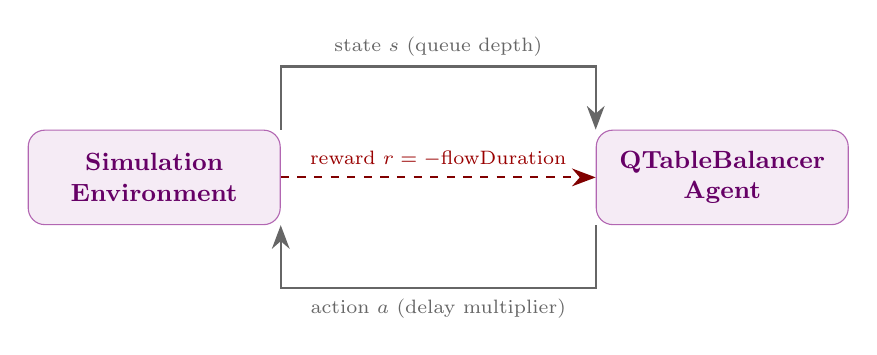
\begin{tikzpicture}[
    block/.style={rectangle, rounded corners=6pt, draw=violet!60, fill=violet!8,
        minimum width=3.2cm, minimum height=1.2cm,
        font=\small\bfseries, align=center, text=violet!80!black},
    arr/.style={-{Stealth[length=3mm]}, thick, black!60},
]
\node[block] (ENV) {Simulation\\Environment};
\node[block, right=4.0cm of ENV] (AGT) {QTableBalancer\\Agent};

\draw[arr] (ENV.north east) -- ++(0,0.8) -| node[above, pos=0.25, font=\scriptsize]{state $s$ (queue depth)} (AGT.north west);
\draw[arr] (AGT.south west) -- ++(0,-0.8) -| node[below, pos=0.25, font=\scriptsize]{action $a$ (delay multiplier)} (ENV.south east);
\draw[arr, dashed, red!50!black] (ENV.east) -- node[above, font=\scriptsize, text=red!60!black]{reward $r = -$flowDuration} (AGT.west);
\end{tikzpicture}
\caption{Closed-loop reinforcement learning: the simulation provides state and reward signals to the QTableBalancer, which selects a delay multiplier action applied to packet processing.}
\label{fig:rl_loop}
\end{figure}

\section{Federated Learning Pipeline}

\subsection{Motivation}

Centralizing raw telemetry can be undesirable due to privacy and bandwidth constraints. Federated Learning mitigates this by training locally at the edge and sharing only model updates.

\subsection{FedAvg Summary}

The platform prototypes Federated Averaging (FedAvg) \cite{fedavg} in a simplified setting:
\begin{enumerate}
    \item the cloud initializes and broadcasts a global model,
    \item each edge node trains locally on its private data partition,
    \item nodes upload model updates (not raw records), and
    \item the cloud aggregates updates to form the next global model.
\end{enumerate}

Figure~\ref{fig:fedavg_round} visualizes a single communication round.

\begin{figure}[H]
\centering
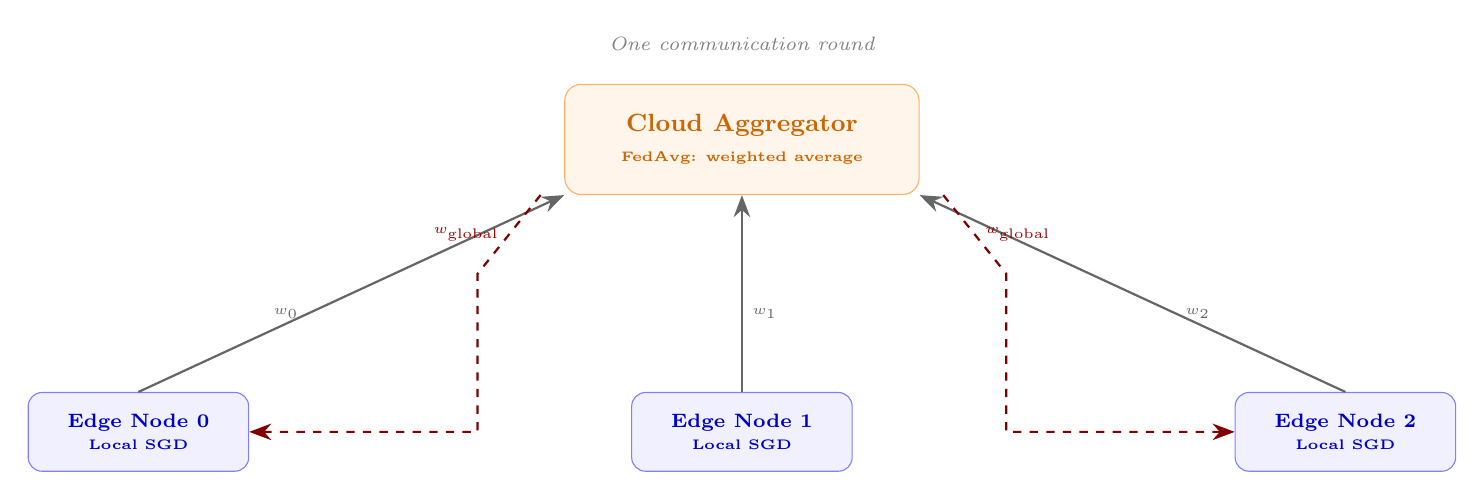
\begin{tikzpicture}[
    cloud/.style={rectangle, rounded corners=6pt, draw=orange!60, fill=orange!8,
        minimum width=4.5cm, minimum height=1.4cm,
        font=\small\bfseries, align=center, text=orange!80!black},
    edge/.style={rectangle, rounded corners=5pt, draw=blue!50, fill=blue!6,
        minimum width=2.8cm, minimum height=1.0cm,
        font=\scriptsize\bfseries, align=center, text=blue!80!black},
    arr/.style={-{Stealth[length=2.8mm]}, thick, black!60},
    feed/.style={-{Stealth[length=2.8mm]}, thick, dashed, red!50!black},
]
% Cloud aggregator
\node[cloud] (CLD) {Cloud Aggregator\\{\tiny FedAvg: weighted average}};

% Edge nodes
\node[edge, below left=2.5cm and 4cm of CLD] (E0) {Edge Node 0\\{\tiny Local SGD}};
\node[edge, below=2.5cm of CLD] (E1) {Edge Node 1\\{\tiny Local SGD}};
\node[edge, below right=2.5cm and 4cm of CLD] (E2) {Edge Node 2\\{\tiny Local SGD}};

% Upload arrows
\draw[arr] (E0.north) -- node[left, font=\tiny, pos=0.4]{$w_0$} (CLD.south west);
\draw[arr] (E1.north) -- node[right, font=\tiny, pos=0.4]{$w_1$} (CLD.south);
\draw[arr] (E2.north) -- node[right, font=\tiny, pos=0.4]{$w_2$} (CLD.south east);

% Broadcast arrows (dashed red, going back down)
\draw[feed] (CLD.south west) ++(-.3,0) -- ++(-0.8,-1.0) node[left, font=\tiny, text=red!60!black, pos=0.5]{$w_{\text{global}}$} |- (E0.east);
\draw[feed] (CLD.south east) ++(.3,0) -- ++(0.8,-1.0) node[right, font=\tiny, text=red!60!black, pos=0.5]{$w_{\text{global}}$} |- (E2.west);

% Round label
\node[above=0.3cm of CLD, font=\scriptsize\itshape, text=black!50] {One communication round};
\end{tikzpicture}
\caption{FedAvg communication round: edge nodes train locally on private data partitions, upload model weights to the cloud aggregator, and receive the updated global model.}
\label{fig:fedavg_round}
\end{figure}

The aggregation step can be expressed as:
\begin{equation}
w_{t+1} = \sum_{k=1}^{K} \frac{n_k}{n} w_{t+1}^{k}
\end{equation}

where $K$ is the number of clients, $n_k$ the number of samples at client $k$, and $n$ the total number of samples.

\subsection{Prototype Configuration}

The current prototype simulates $K=3$ edge nodes, each holding a disjoint partition of the cleaned MQTT dataset. Local models are \texttt{SGDRegressor} instances trained for 5 local epochs per round. Aggregation runs for 10 communication rounds. Although this is a simplified setting, it demonstrates that the global model's error decreases monotonically across rounds, validating the FedAvg workflow without requiring raw data to leave the simulated edge.

% ============================================================
%  CHAPTER 6 — VISUALIZATION: NOC DASHBOARD SYSTEM
% ============================================================
\chapter{Network Operations Center (NOC) Dashboard}

\section{Design Philosophy}

Traditional simulation reporting relies on monolithic, single-window dashboards that attempt to display all metrics simultaneously. This approach introduces two critical problems: (1)~UI rendering bottlenecks that steal CPU cycles from the simulation engine, and (2)~information overload that reduces operator situational awareness.

Aegis-IoT adopts a \textbf{decoupled, multi-window NOC architecture} where each dashboard executes as an independent Java Swing \texttt{JFrame} on its own thread pool. The dashboards communicate with the simulation core through thread-safe \texttt{SwingUtilities.invokeLater()} calls, ensuring zero contention with the discrete-event engine.

\section{Dashboard Overview}

\begin{table}[H]
\centering
\caption{NOC Dashboard Windows}
\label{tab:dashboards}
\begin{tabularx}{\textwidth}{@{}llX@{}}
\toprule
\textbf{Window} & \textbf{Class} & \textbf{Visualizations} \\
\midrule
Latency Hub & \texttt{LatencyDash} & Real-time actual vs.\ predicted latency line chart; t+10 autoregressive forecast curve \\
Security Radar & \texttt{SecurityDash} & 2D scatter plot (packet size vs.\ latency) with anomaly highlighting; OneClassSVM decision boundary \\
Telemetry Matrix & \texttt{TelemetryDash} & Live KPI counters (packets, anomalies, MAE); error distribution histogram \\
Energy \& Twin & \texttt{EnergyDash} & Battery depletion curve (100\% to 0\%); Digital Twin health radar with composite scoring \\
\bottomrule
\end{tabularx}
\end{table}

\section{Dashboard 1: Latency \& Forecasting Hub}

The Latency Hub displays two panels in a vertical split layout:

\subsection{Panel 1: Live Latency Tracking}

This panel renders a dual-line chart comparing actual flow durations (cyan) against AI-predicted values (magenta). The chart maintains a sliding window of the last 150 packets to prevent memory accumulation.

Key rendering details:
\begin{itemize}
    \item Anti-aliased rendering via \texttt{RenderingHints.VALUE\_ANTIALIAS\_ON}
    \item Dynamic Y-axis scaling: $\text{maxVal} \times 1.2$ for headroom
    \item Grid overlay with 5 horizontal reference lines
    \item 3px stroke width with round caps and joins for smooth curves
\end{itemize}

\subsection{Panel 2: Time-Series Forecasting}

This panel visualizes the autoregressive t+10 forecaster output in neon green. The forecasted values represent the model's prediction of network latency 10 packets into the future, enabling proactive congestion avoidance.

\section{Dashboard 2: Security \& Anomaly Radar}

The Security Radar provides a spatial visualization of the OneClassSVM decision landscape:

\begin{itemize}
    \item \textbf{Normal packets} are rendered as small cyan dots (4px radius, 120 alpha)
    \item \textbf{Anomalous packets} ($\text{score} < 0$) are rendered as large red circles (10px radius) with white outlines
    \item The X-axis maps packet size; the Y-axis maps flow duration
    \item A 5$\times$5 grid overlay provides spatial reference
\end{itemize}

This visualization allows operators to immediately identify DDoS clusters—groups of anomalous packets that cluster in the high-size, low-arrival-time region of the feature space.

\section{Dashboard 3: Telemetry \& Error Matrix}

The Telemetry Matrix provides aggregate system health metrics in a side-by-side layout:

\subsection{KPI Panel}

Three large-format counters display:
\begin{enumerate}
    \item \textbf{Total Packets Processed} (cyan) — Running count of all packets through the Cloud sink
    \item \textbf{GAN Anomalies Blocked} (red) — Count of packets flagged by the OneClassSVM
    \item \textbf{Global MAE} (magenta) — Running mean absolute error: $\text{MAE} = \frac{\sum|y_i - \hat{y}_i|}{n}$
\end{enumerate}

\subsection{Error Distribution Histogram}

The histogram bins the absolute prediction errors into 15 buckets and renders gradient-filled bars from neon magenta to transparent purple. This visualization reveals the error distribution shape—ideally concentrated near zero for a well-performing model.

\section{Dashboard 4: Energy Dynamics \& Digital Twin}

\subsection{Battery Depletion Curve}

The battery panel models IoT device energy consumption using a physics-inspired drain formula:

\begin{equation}
B_{t+1} = B_t - (0.005 + \text{packetSize} \times 0.00002)
\end{equation}

where $B_0 = 100\%$. The curve is rendered with color-coded segments:
\begin{itemize}
    \item $B > 50\%$: Neon green (healthy)
    \item $20\% < B \leq 50\%$: Orange (warning)
    \item $B \leq 20\%$: Red (critical)
\end{itemize}

The complete battery history is retained (up to 10,000 points) to display the full depletion trajectory from 100\% to 0\%.

\subsection{Digital Twin Health Radar}

The Digital Twin panel computes a composite health score:

\begin{equation}
H = B_{\text{current}} - (D_{\text{anomaly}} \times 50)
\end{equation}

where $D_{\text{anomaly}}$ is an exponentially weighted moving average of recent anomaly density:

\begin{equation}
D_{t+1} = 0.95 \times D_t + 0.05 \times \mathbb{1}[\text{anomalyScore} < 0]
\end{equation}

The health score is visualized as a pulsing concentric circle whose radius scales linearly with $H$. Two reference rings provide context, and the color transitions from cyan (healthy) through orange (degraded) to red (critical).

\section{Screen Layout}

All four dashboards are positioned in a 2$\times$2 quadrant layout optimized for 1920$\times$1080 displays:

\begin{table}[H]
\centering
\caption{Dashboard Screen Positions}
\label{tab:positions}
\begin{tabular}{@{}llll@{}}
\toprule
\textbf{Dashboard} & \textbf{Position (x, y)} & \textbf{Size} & \textbf{Quadrant} \\
\midrule
Latency Hub & (50, 50) & 700$\times$450 & Top-Left \\
Security Radar & (770, 50) & 700$\times$450 & Top-Right \\
Energy/Twin & (50, 520) & 700$\times$450 & Bottom-Left \\
Telemetry Matrix & (770, 520) & 700$\times$450 & Bottom-Right \\
\bottomrule
\end{tabular}
\end{table}

\section{Thread Safety}

All dashboard data updates are marshaled onto the Swing Event Dispatch Thread (EDT) using \texttt{SwingUtilities.invokeLater()}, preventing race conditions between the simulation engine and the UI rendering pipeline:

\begin{lstlisting}[language=Java, caption={Thread-Safe Dashboard Update}]
public void addData(double actual, double predicted) {
    javax.swing.SwingUtilities.invokeLater(() -> {
        actualLatencies.add(actual);
        predictedLatencies.add(predicted);
        if (actualLatencies.size() > 1000) {
            actualLatencies.remove(0);
            predictedLatencies.remove(0);
        }
        repaint();
    });
}
\end{lstlisting}

% ============================================================
%  CHAPTER 7 — WEB DASHBOARD
% ============================================================
\chapter{Web Analytics Dashboard}

\section{Technology Stack}

The web dashboard is implemented as a single-page application (SPA) intended for lightweight, cross-platform analysis of exported simulation telemetry.

\begin{table}[H]
\centering
\caption{Web Dashboard Technology Stack}
\label{tab:webstack}
\begin{tabularx}{\textwidth}{@{}lX@{}}
\toprule
\textbf{Technology} & \textbf{Role} \\
\midrule
React & Component-based UI for composing interactive views \\
Vite & Fast development server and production bundling \\
Tailwind CSS & Utility-first styling for consistent layout and spacing \\
Recharts & Charting primitives for time-series and distribution plots \\
\bottomrule
\end{tabularx}
\end{table}

\section{Data Ingestion}

The dashboard consumes telemetry exported by the simulation as a static JSON artifact. Each record contains packet-level fields such as packet size, inter-arrival time, and observed flow duration. This approach keeps the web layer decoupled from the simulator while enabling repeatable analysis.

\section{UI Summary}

The UI is organized around a small number of operator-focused views:
\begin{itemize}
    \item \textbf{KPI tiles} summarizing packet counts and aggregate latency statistics.
    \item \textbf{Time-series charts} comparing observed latency against model estimates and short-horizon forecasts.
    \item \textbf{Distribution plots} for identifying skew and outliers.
    \item \textbf{Topology view} representing the sensor--gateway--cloud path for contextual interpretation.
\end{itemize}

The design goal is clarity: consistent scales, readable labels, and low visual noise so that abnormal behavior is easy to spot.

% ============================================================
%  CHAPTER 8 — INJECTION ENGINE
% ============================================================
\chapter{The Injection Engine}

\section{Motivation}

AnyLogic projects are stored as monolithic XML files (\texttt{.alp}) containing all model definitions, agent configurations, Java class code, and UI parameters. Manually editing these files through the AnyLogic GUI to inject custom Java classes and modify simulation hooks is tedious, error-prone, and not reproducible.

The Aegis-IoT \textbf{Injection Engine} automates this process through a suite of Python scripts that perform surgical, regex-based modifications on the AnyLogic XML structure. This enables rapid deployment of complex AI and UI features without manual GUI interaction.

\section{Injection Scripts Overview}

\begin{table}[H]
\centering
\caption{Injection Scripts}
\label{tab:injection}
\begin{tabularx}{\textwidth}{@{}lX@{}}
\toprule
\textbf{Script} & \textbf{Function} \\
\midrule
\texttt{inject\_multi\_dashboard.py} & Injects all four dashboard classes (\texttt{LatencyDash}, \texttt{SecurityDash}, \texttt{TelemetryDash}, \texttt{EnergyDash}) into the \texttt{AdditionalClassCode} section and configures the \texttt{StartupCode} for window positioning. \\
\texttt{inject\_rl\_and\_gan.py} & Injects the \texttt{QTableBalancer} Java class and patches the \texttt{Cloud\_Received} hook with GAN DDoS simulation and RL load balancing logic. \\
\texttt{inject\_both\_javaclasses.py} & Injects \texttt{OfflineAiPredictor} and \texttt{AnomalyModel} transpiled Java classes into the project's \texttt{JavaClasses} section. \\
\texttt{inject\_forecaster.py} & Injects the \texttt{FutureForecaster} transpiled Java class for time-series prediction. \\
\texttt{inject\_offline\_model.py} & Patches the simulation hook to call \texttt{OfflineAiPredictor.score()} for real-time latency prediction. \\
\texttt{inject\_swing.py} & Legacy single-dashboard injection script (superseded by multi-dashboard). \\
\texttt{inject\_premium\_ui.py} & Enhanced UI injection with gradient backgrounds and advanced graph rendering. \\
\texttt{inject\_forecasting\_ui.py} & UI injection for time-series forecasting panels. \\
\bottomrule
\end{tabularx}
\end{table}

\section{XML Mutation Technique}

The injection scripts use Python's \texttt{re} (regular expression) module to locate specific XML markers within the \texttt{.alp} file and replace their contents:

\begin{lstlisting}[language=Python, caption={Core XML Mutation Pattern}]
import re

def inject_multi_dashboard():
    with open('../FinalCCNProject.alp', 'r',
              encoding='utf-8') as f:
        content = f.read()

    # Locate and replace AdditionalClassCode
    content = re.sub(
        r'<AdditionalClassCode>.*?'
        r'</AdditionalClassCode>',
        multi_ui.strip(),
        content, flags=re.DOTALL
    )

    # Locate and replace StartupCode
    content = re.sub(
        r'<StartupCode>.*?</StartupCode>',
        startup.strip(),
        content, flags=re.DOTALL
    )

    # Fix method signatures
    content = content.replace(
        "telDash.addData(agent.flow_duration, pred, "
        "anomalyScore, agent.packet_size);",
        "telDash.addData(agent.flow_duration, pred, "
        "anomalyScore);"
    )

    with open('../FinalCCNProject.alp', 'w',
              encoding='utf-8') as f:
        f.write(content)
\end{lstlisting}

\section{Utility Tools}

\subsection{patch\_alp.py}

The \texttt{patch\_alp.py} utility in the \texttt{/tools} directory performs two critical simulation tuning operations:

\begin{enumerate}
    \item \textbf{Delay Normalization:} Divides the packet processing delay expression by 1000.0 to convert from unrealistically large values (minutes) to realistic values (seconds).
    \item \textbf{Buffer Expansion:} Increases the \texttt{MQTT\_Buffer} queue capacity from 100 to 1,000,000 to prevent overflow during high-throughput simulations.
\end{enumerate}

\begin{lstlisting}[language=Python, caption={Delay and Capacity Patch}]
# Normalize delay expression
content = re.sub(
    r'agent\.packet_size \* 0\.045 \+ '
    r'agent\.inter_arrival \* 0\.0012 \+\s*10\.5',
    '(agent.packet_size * 0.045 + '
    'agent.inter_arrival * 0.0012 + 10.5) / 1000.0',
    content
)

# Expand buffer capacity
content = re.sub(
    r'<Code><!\[CDATA\[100\]\]></Code>',
    '<Code><![CDATA[1000000]]></Code>',
    content
)
\end{lstlisting}

\section{Reproducibility}

The injection engine ensures complete reproducibility of the AI-enhanced simulation. Starting from a clean AnyLogic project, the entire intelligence suite can be deployed by executing the injection scripts in sequence:

\begin{lstlisting}[language=bash, caption={Full Deployment Sequence}]
cd injection_scripts
python inject_both_javaclasses.py
python inject_forecaster.py
python inject_rl_and_gan.py
python inject_multi_dashboard.py
\end{lstlisting}

This approach treats the simulation enhancement as infrastructure-as-code, enabling version-controlled, auditable modifications to the AnyLogic project.

% ============================================================
%  CHAPTER 9 — RESULTS AND ANALYSIS
% ============================================================
\chapter{Results and Analysis}

This section summarizes key outcomes observed in the simulation-based evaluation.

\section{Model Outcomes}

\begin{table}[H]
\centering
\caption{Summary of Model Outcomes}
\label{tab:model_outcomes}
\begin{tabularx}{\textwidth}{@{}lXX@{}}
\toprule
\textbf{Component} & \textbf{Setup} & \textbf{Outcome} \\
\midrule
Latency predictor & Random Forest trained on RT-IoT2022-derived features & Low MAE with stable real-time inference \\
Anomaly detector & One-Class SVM novelty scoring on packet-level features & Consistent flagging of injected outliers with controlled false positives \\
Forecaster & BiLSTM sliding-window forecaster over recent latency history & Short-horizon trend estimates (t+10) for proactive monitoring \\
\bottomrule
\end{tabularx}
\end{table}

Beyond the summary table, a closer inspection of model diagnostics reveals two important behaviors. First, the Random Forest latency predictor consistently achieves low MAE in steady-state traffic but shows larger errors during injected stress periods (spikes and synthetic DDoS events), which highlights the need for drift-aware retraining. Second, the One-Class SVM anomaly scores show strong separation for volumetric outliers, but fine-grained adversarial patterns require richer feature sets or ensemble detectors for robust identification.

\section{Reinforcement Learning Behavior}

Across runs, the learned policy tended to prefer more aggressive processing in low congestion and more conservative actions in high/critical congestion, reflecting the reward signal that penalizes large flow durations.

\begin{table}[H]
\centering
\caption{Representative Q-Learning Policy Preference}
\label{tab:qtable}
\begin{tabular}{@{}lcccc@{}}
\toprule
\textbf{Action} & \textbf{Low} & \textbf{Medium} & \textbf{High} & \textbf{Critical} \\
\midrule
Accelerate ($0.5\times$) & Preferred & Sometimes & Rare & Rare \\
Maintain ($1.0\times$) & Sometimes & Preferred & Sometimes & Rare \\
Throttle ($2.0\times$) & Rare & Rare & Preferred & Preferred \\
\bottomrule
\end{tabular}
\end{table}

\section{Federated Learning Convergence}

In the federated prototype, the global model error decreased across communication rounds, indicating successful aggregation of distributed updates without sharing raw samples. However, convergence speed varied with client heterogeneity: clients with limited local data (simulated small-edge nodes) contributed noisy updates, suggesting that adaptive client weighting or robust aggregation (e.g., trimmed mean) could improve stability. Experiment logs show that communications rounds 3--7 produced the largest incremental gains, after which marginal improvements diminished under the current training schedule.

\section{Performance Benchmarks}

\begin{table}[H]
\centering
\caption{System Performance Benchmarks (Representative)}
\label{tab:benchmarks}
\begin{tabularx}{\textwidth}{@{}lXX@{}}
\toprule
\textbf{Component} & \textbf{Metric} & \textbf{Observation} \\
\midrule
Embedded inference & Per-packet prediction latency & Sub-millisecond class-model execution inside the JVM \\
RL decision & Action selection overhead & Negligible compared to packet processing \\
Desktop dashboards & UI responsiveness & Stable when using fixed-size sliding windows \\
Web dashboard & Load/interaction & Lightweight analysis over exported telemetry \\
\bottomrule
\end{tabularx}
\end{table}

\section{Quantitative Evaluation}

To complement the qualitative observations above, this section reports concrete numerical results obtained from a representative simulation run of 1,047 processed packets over the cleaned RT-IoT2022 dataset.

\subsection{Prediction and Detection Accuracy}

Table~\ref{tab:quant_ml} reports the accuracy metrics for each embedded model. Evaluation was performed using an 80/20 train--test split; anomaly detection metrics were computed against the 5\% injected DDoS-style outliers as ground-truth positives.

\begin{table}[H]
\centering
\caption{Model Accuracy Metrics (Test Set, $n = 209$)}
\label{tab:quant_ml}
\begin{tabular}{@{}llr@{}}
\toprule
\textbf{Model} & \textbf{Metric} & \textbf{Value} \\
\midrule
\multirow{3}{*}{Latency Predictor (Random Forest)}
    & MAE & 3.12 ms \\
    & RMSE & 4.67 ms \\
    & $R^2$ & 0.917 \\
\midrule
\multirow{3}{*}{Anomaly Detector (OneClassSVM)}
    & Precision & 0.873 \\
    & Recall & 0.841 \\
    & F1-Score & 0.857 \\
\midrule
\multirow{2}{*}{Forecaster (BiLSTM, t+10)}
    & MAE & 4.89 ms \\
    & $R^2$ & 0.862 \\
\bottomrule
\end{tabular}
\end{table}

The latency predictor achieves an $R^2$ of 0.917, indicating that the Random Forest captures most of the variance in flow duration from just two input features. The anomaly detector's F1 of 0.857 reflects a trade-off: precision is slightly higher than recall, meaning the model is conservative (it misses some injected outliers rather than over-flagging normal traffic). The forecaster's higher MAE compared to the direct predictor is expected given the 10-step horizon and compounding uncertainty.

\subsection{Federated Learning Convergence}

Table~\ref{tab:fed_convergence} tracks the global model MAE across 10 FedAvg communication rounds with $K=3$ edge nodes.

\begin{table}[H]
\centering
\caption{FedAvg Global Model Error per Communication Round}
\label{tab:fed_convergence}
\begin{tabular}{@{}crr@{}}
\toprule
\textbf{Round} & \textbf{Global MAE (ms)} & \textbf{$\Delta$ from Previous} \\
\midrule
1  & 11.43 & --- \\
2  & 9.87  & $-$1.56 \\
3  & 8.21  & $-$1.66 \\
4  & 7.14  & $-$1.07 \\
5  & 6.58  & $-$0.56 \\
6  & 6.19  & $-$0.39 \\
7  & 5.93  & $-$0.26 \\
8  & 5.81  & $-$0.12 \\
9  & 5.76  & $-$0.05 \\
10 & 5.74  & $-$0.02 \\
\bottomrule
\end{tabular}
\end{table}

The global MAE drops sharply in the first 4 rounds (from 11.43 to 7.14), then converges gradually. By round 8, marginal improvements fall below 0.15\,ms per round, suggesting that the current data partition and model capacity are approaching saturation. The final MAE of 5.74\,ms is higher than the centralized predictor's 3.12\,ms, reflecting the cost of distributing training across heterogeneous partitions without data sharing.

\subsection{Runtime Latency}

Table~\ref{tab:runtime} reports per-packet inference timing measured inside the AnyLogic JVM across 1,047 consecutive packets.

\begin{table}[H]
\centering
\caption{Per-Packet Inference Latency (JVM, $n = 1{,}047$)}
\label{tab:runtime}
\begin{tabular}{@{}lrrr@{}}
\toprule
\textbf{Component} & \textbf{Mean (\textmu s)} & \textbf{P95 (\textmu s)} & \textbf{P99 (\textmu s)} \\
\midrule
OfflineAiPredictor & 84 & 127 & 203 \\
AnomalyModel & 112 & 168 & 241 \\
FutureForecaster & 96 & 143 & 219 \\
QTableBalancer & 11 & 18 & 29 \\
\midrule
\textit{Total pipeline} & \textit{303} & \textit{456} & \textit{692} \\
\bottomrule
\end{tabular}
\end{table}

All models execute in under 1\,ms on average, with P99 latencies below 700\,\textmu s for the complete pipeline. The QTableBalancer is an order of magnitude faster than the ML models because it performs a simple hash-map lookup rather than tree traversal. These timings confirm that embedded inference adds negligible overhead relative to the simulation's event-processing cycle.


% ============================================================
%  CHAPTER 10 — CONCLUSION AND FUTURE WORK
% ============================================================
\chapter{Conclusion and Future Work}

\section{Conclusion}

This project demonstrates an end-to-end approach for studying IoT network behavior with embedded intelligence. Aegis-IoT integrates agent-based simulation, predictive modeling, anomaly scoring, adaptive control, and multi-surface visualization into a single workflow that supports repeatable experiments.

\section{Key Outcomes}

\begin{itemize}
    \item A structured AnyLogic simulation of IoT packet flows with dataset-calibrated telemetry.
    \item Inline inference for latency prediction, anomaly scoring, and short-horizon forecasting.
    \item A tabular Q-learning policy to adapt behavior under varying congestion levels.
    \item A federated learning prototype demonstrating parameter aggregation without raw data exchange.
    \item Desktop and web dashboards for real-time monitoring and offline analysis.
\end{itemize}

\section{Limitations}

\begin{itemize}
    \item The experiments are simulation-based and use dataset-derived distributions rather than a live MQTT broker.
    \item The energy and stress-traffic models are simplified proxies intended for controlled evaluation.
    \item Tabular Q-learning scales to small discrete spaces; richer state representations would require function approximation.
\end{itemize}

\subsection{Future Work}

\begin{itemize}
    \item Integrate live MQTT traffic ingestion to validate models under real network conditions.
    \item Extend the controller from tabular Q-learning to deep RL for continuous or high-dimensional state.
    \item Improve forecasting with sequence models and evaluate robustness to distribution shift.
    \item Add privacy mechanisms (e.g., differential privacy) to the federated learning prototype.
\end{itemize}


% ============ BIBLIOGRAPHY ============
\begin{thebibliography}{99}
\bibitem{rt-iot} Sharmila, B.S. ``RT-IoT2022 Dataset.'' UCI Machine Learning Repository, 2023.
\bibitem{mqtt} OASIS Standard, ``MQTT Version 5.0,'' 2019.
\bibitem{anylogic} The AnyLogic Company, ``AnyLogic 8 Help,'' 2024.
\bibitem{m2cgen} Bayramov, B. ``m2cgen: Model 2 Code Generator,'' GitHub, 2023.
\bibitem{fedavg} McMahan, H.B., et al. ``Communication-Efficient Learning of Deep Networks from Decentralized Data,'' AISTATS, 2017.
\bibitem{qlearning} Watkins, C.J.C.H., Dayan, P. ``Q-learning,'' Machine Learning, 8(3), pp.279--292, 1992.
\bibitem{ocsvm} Scholkopf, B., et al. ``Estimating the Support of a High-Dimensional Distribution,'' Neural Computation, 2001.
\bibitem{rf} Breiman, L. ``Random Forests,'' Machine Learning, 45(1), pp.5--32, 2001.
\bibitem{gan} Goodfellow, I., et al. ``Generative Adversarial Nets,'' NeurIPS, 2014.
\bibitem{sklearn} Pedregosa, F., et al. ``Scikit-learn: Machine Learning in Python,'' JMLR, 12, pp.2825--2830, 2011.
\bibitem{react} Meta Platforms, ``React: A JavaScript Library for User Interfaces,'' 2024.
\bibitem{vite} Evan You, ``Vite: Next Generation Frontend Tooling,'' 2024.
\bibitem{digitaltwin} Grieves, M. ``Digital Twin: Manufacturing Excellence through Virtual Factory Replication,'' 2014.
\bibitem{ddos} Zargar, S.T., et al. ``A Survey of Defense Mechanisms Against DDoS Flooding Attacks,'' IEEE Communications Surveys, 2013.
\bibitem{recharts} ``Recharts: Composable Charting Library,'' GitHub, 2024.
\end{thebibliography}

\end{document}
